\documentclass[11pt,a4paper]{article}
\usepackage{graphicx}
\usepackage{subcaption}
\author{Horacio Hoyos Rodriguez}
\title{NBody Simulation with Crossflow}

\begin{document}

\maketitle
    
\section{Introduction}
The aim of the exercise was to see if we could use \emph{Crossflow} to process time-consuming physics simulations.
The test simulation was the NBody problem, where we want to predict the individual motions of a group of celestial objects interacting with each other gravitationally.
The objectives where:
\begin{itemize}
    \item Find a way of representing the problem so that it was amenable to be executed in a distirbuted architecture
    \item Determine if using Crossflow could result in significant performance gains. 
\end{itemize}

To meet this objectives I focused on three main activities:
\begin{enumerate}
    \item Write a Java version of the provided NBody simulation example written in C.
    \item Develop an Object-oriented (OO) version of the simulation.
    \item Develop a multi-threaded version of the simulation.
    \item Develop a Crossflow version of the simulation.
\end{enumerate}

Activity (1) was to make sure we understood the code and got similar results (given the randomization of the initial positions).
Activity (2) helped us structure the code in a way that is more amenable for splitting into smaller parts.
With the results from (2), activity (3) would help us understand what changes where needed for a ``distributed'' execution; mainly how to share information between objects running different parts of the simulation.
Finally, the ideas from (3) where used to build (4).

\section{Implementations}
\subsection{C clone}
The first implementation was a clone, almost line by line of the provided C example.
A few minor tweaks where required to migrate some C libs and constructs to Java.
Further, we also cloned the OpenGL code, so we could actually visualize the simulation.
The hardest part was the OpenGL stuff.

\subsection{Object-oriented}
The Object-oriented implementation introduced classes to represent a vector (each of the bodies) and a cuboid (which holds a subset of the total bodies).
The vector class is responsible for all the vector operations (add, multiple, etc.).
The cuboid class is responsible for simulating (calculate new acceleration and velocity, and final position of all bodies inside the cuboid).
The cuboid is also responsible for time and memory measurements.
Currently, we only support axis-aligned cuboids.
In this implementation, we have a single cuboid that represents the complete space.

\subsection{Multi-threaded}
In this implementation we can run the simulation via multiple threads.
The general idea is that we can divide the complete space into into \emph{n} number of cuboids (\emph{n} has to be a power of 2) and each of these cuboids can be simulated (per step) in a separate thread.
A per-step control is required as we need the results of the complete space at step $j-1$ in order to simulate step $j$.

A master thread is responsible for coordination: synchronize steps and distribute information.
A runner is responsible for simulating one cuboid for one step in a thread.
For each step, the master creates $n$ cuboids and makes them available to a set of runners (via a queue).
Each runner takes a cuboid from the queue, simulates a step and sends the results to the master (via a queue).
The results include the new body information for each body in the cuboid and the time information.
Note that a single runner could run multiple queues.
Further, the master could change $n$ at any step.

\subsection{Crossflow}
The Crossflow implementation is an extension of the multi-threaded version, to adjust the master and workers to use crossflow queues.
Figure\,\ref{fig:nbody} presents the diagram of the crossflow version of the NBody problem.

\begin{figure}
    \centering
    \includegraphics[width=0.9\linewidth]{nbody}
    \caption{Crossflow NBody diagram}
    \label{fig:nbody}
\end{figure}

The \emph{Experiment} source allows the crossflow to execute multiple experiments.
Each experiment consists of the number of bodies and the number of steps in the simulation.
The \emph{Lines} queue is used to send experiment information to the Step task.

The \emph{Step} task is responsible for controlling the execution of the experiment.
Its functionality is very similar to the mater thread in the multi-threaded version.
At each step, the task creates a \texttt{StepData} message for each cuboid; the number of cuboids is fixed for each experiment (and provided as part of the experiment information).
The \texttt{StepData} message also contains information about the current state of the complete space (\emph{universe}), simulation information (veloicty dampening and timestep) and if the Simulation tasks should use multi-threads.

The \emph{Simulation} task is responsible for simulating a single step for a given cuboid.
In this respect, it behaves as a runner in the multi-threaded version as it consumes cuboids from the Universe queue.
However, if the \texttt{threaded} field in the \texttt{StepData} message is set to \emph{true}, then the Simluation step will behave as multi-thread master, dividing the cuboid into more cuboids (depending on the number of available cores) and spawning runners to simulate the step.
After simulating the step, the \emph{Simulation} task will send the results to the Step task.

After all steps have been completed, the \emph{Step} task sends the results to the Performance queue which in turn is used by the Data sink to persist them to file.
   
\section{Results}

Note that these results are very preliminary and probably need a more proper setup (not possible due to time constraints).
In all cases the phi/hash of the results was stored, and we verified that they all got the same result.
All simulations where done over 100 steps, with 10, 100, 1k, 10k and 100k bodies.

\subsection{Single Applications}

\begin{figure}
    \centering
    \begin{subfigure}{.5\textwidth}
        \centering
        \includegraphics[width=\textwidth]{gflops}
        \caption{Inner MFLOP/s}
        \label{fig:gflops}
    \end{subfigure}%
    \begin{subfigure}{.5\textwidth}
        \centering
        \includegraphics[width=\textwidth]{tgflops}
        \caption{Total MFLOP/s}
        \label{fig:tgflops}
    \end{subfigure}%
\caption{10 iterations of 100 step simulations for different number of bodies.}
\end{figure}

Figure\,\ref{fig:gflops} presents the MFLOP/s measurements for the single application implementations: \emph{cs257} is the C-clone implementation, \emph{simple} is the object-oriented and \emph{threads} is the multi-threaded version.
The MFLOP/s is the measure of (mega) floating-point operations per second.
The time measured corresponds to the inner-most loops that calculate the acceleration, velocity and new position of the bodies, as done in the provided C implementation.
That is, the calculation does not take into consideration the time it takes to process the information, prepare for the next step, etc.
The results suggest that, as expected, the C-clone implementation has a higher throughput than the object-oriented ones.
However, note that the measured time is the \emph{total} time taken doing floating-point arithmetic.
Thus, in a multi-threaded environment even though the computations might be done in parallel their time is added up.

Figure\,\ref{fig:tgflops} presents the FLOPs measure against the total time for the application to run.
In this case, parallel execution times are not added up.
Note that until we go beyond 1000 bodies both the object-oriented implementations outperform the C-clone one.
For 10000 bodies, the results suggest that the multi-threaded implementation is able to keep up with the C-clone.
I didn't manage to get more results for the 100k bodies as it takes about 8 hours to run the simple implementation and 3 hours for the others.

\subsection{Crossflow}

For the crossflow experiment I used one master PC running the workflow and the step tasks.
Three other PC where defined as workers and ran the simulation task.
We also set the \emph{threaded} field of the experiment information to true, so the Simulation workers would take full advantage of the available cores.
I intentionally set the number of experiemnt cuboids to 4, one more than the available workers to see how the workflow behaved.
The consolidated results are presented in Figure\,\ref{fig:crossflow}.

\begin{figure}
    \centering
    \begin{subfigure}{.5\textwidth}
        \centering
        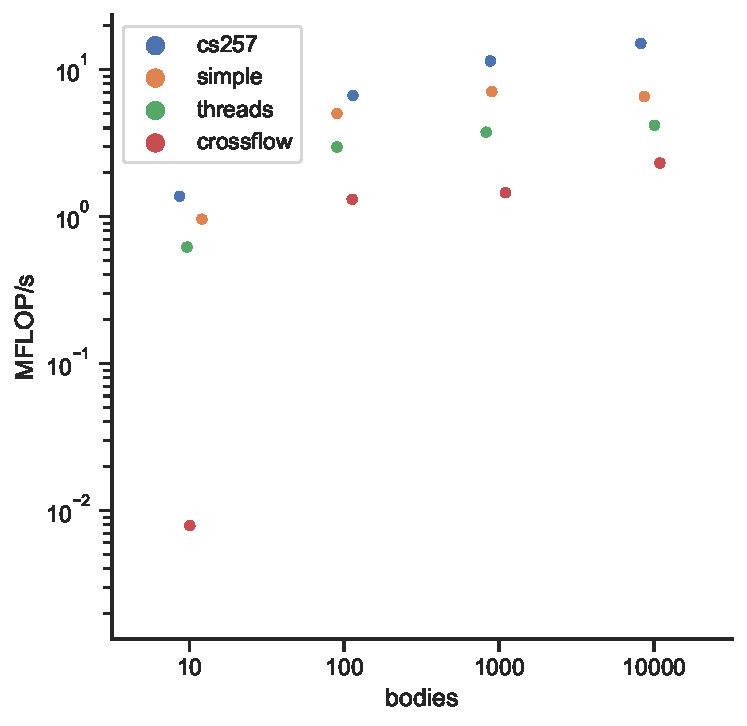
\includegraphics[width=\textwidth]{gflops2}
        \caption{Inner MFLOP/s}
        \label{fig:gflops2}
    \end{subfigure}%
    \begin{subfigure}{.5\textwidth}
        \centering
        \includegraphics[width=\textwidth]{tgflops2}
        \caption{Total MFLOP/s}
        \label{fig:tgflops2}
    \end{subfigure}%
\caption{Consolidated results of 100 step simulations for different number of bodies.}
\label{fig:crossflow}
\end{figure}

The results suggest that the crossflow implementaiton, at the inner loop performance, is around one order of magnitud slower than the cs257 implementation.
The results also suggest that as we increase the number of bodies, the crossflow version tends to come closer to the other implementations.

On the other hand, considering the total time, the results suggest that crossflow is around 2 order of magnitud slower than the other implementations (for $bodies > 100$).
The main reason could be that for each step, the complete state of the simulation (i.e. information of all the bodies) has to be queued and distributed to the workers via an Activemq.

 
\section{Conclusions}
The most significant outcome was to show that it is possible to provide an implementation that allows these type of simulations to run in a Crossflow environment.
The results of the crossflow implementation are encouraging as we have not looked into any further optimizations.
Of these, the most notable could be to store the state of the experiment id a shared resource, for example in a DB, so it does not has to be transmitted via queues.

Other optimizations also can be done to the actual algorithm, which can be found in the literature.

    
\end{document}